
\vspace{1.5cm}


En la figura~\figref{fig:fig_p13_output_impedance} se muestra el gráfico de la impedancia en el nodo de salida en modo de regulación de tensión, el gráfico se obtuvo simulando en \textbf{SPICE} con $R_{L} = 100 \si[per-mode=symbol]{\ohm}$, con una fuente de corriente de señal conectada en paralelo con la carga, $I_{p}$, realizando un barrido en alterna de $0.1 \si[per-mode=symbol]{\hertz}$ a $100 \si[per-mode=symbol]{\kilo\hertz}$, con el comando \textbf{SPICE} \textit{.ac}, y luego obteniendo el cociente $\frac{V\left(I_{p}\right)}{I_{p}}$, el resultado se exportó y se graficó en \textbf{MATLAB}, en escala semilogarítmica, su módulo y su fase, se destacó el resultado a bajas frecuencias que representa la resistencia de salida a frecuencia bajas/medias. El bajo valor obtenido para esta resistencia ($473 \si[per-mode=symbol]{\micro\ohm}$) implica que se trata de una buena fuente de tensión, que en el caso ideal tiene resistencia de salida de $0 \si[per-mode=symbol]{\ohm}$, esto se debe a la gran ganancia de lazo en modo de regulación de tensión. Otra cosa que se puede observar es que al aumentar la frecuencia la impedancia aumenta, al caer la ganancia de lazo, y se torna inductiva, al menos hasta que la fase supera los $90 \si[per-mode=symbol]{\degree}$, esto parece indicar un efecto de resistencia negativa, la fuente entregaría energía de alterna (esto necesita mas análisis).




\vfill

\clearpage

\begin{figure}[H] %htb
\begin{center}
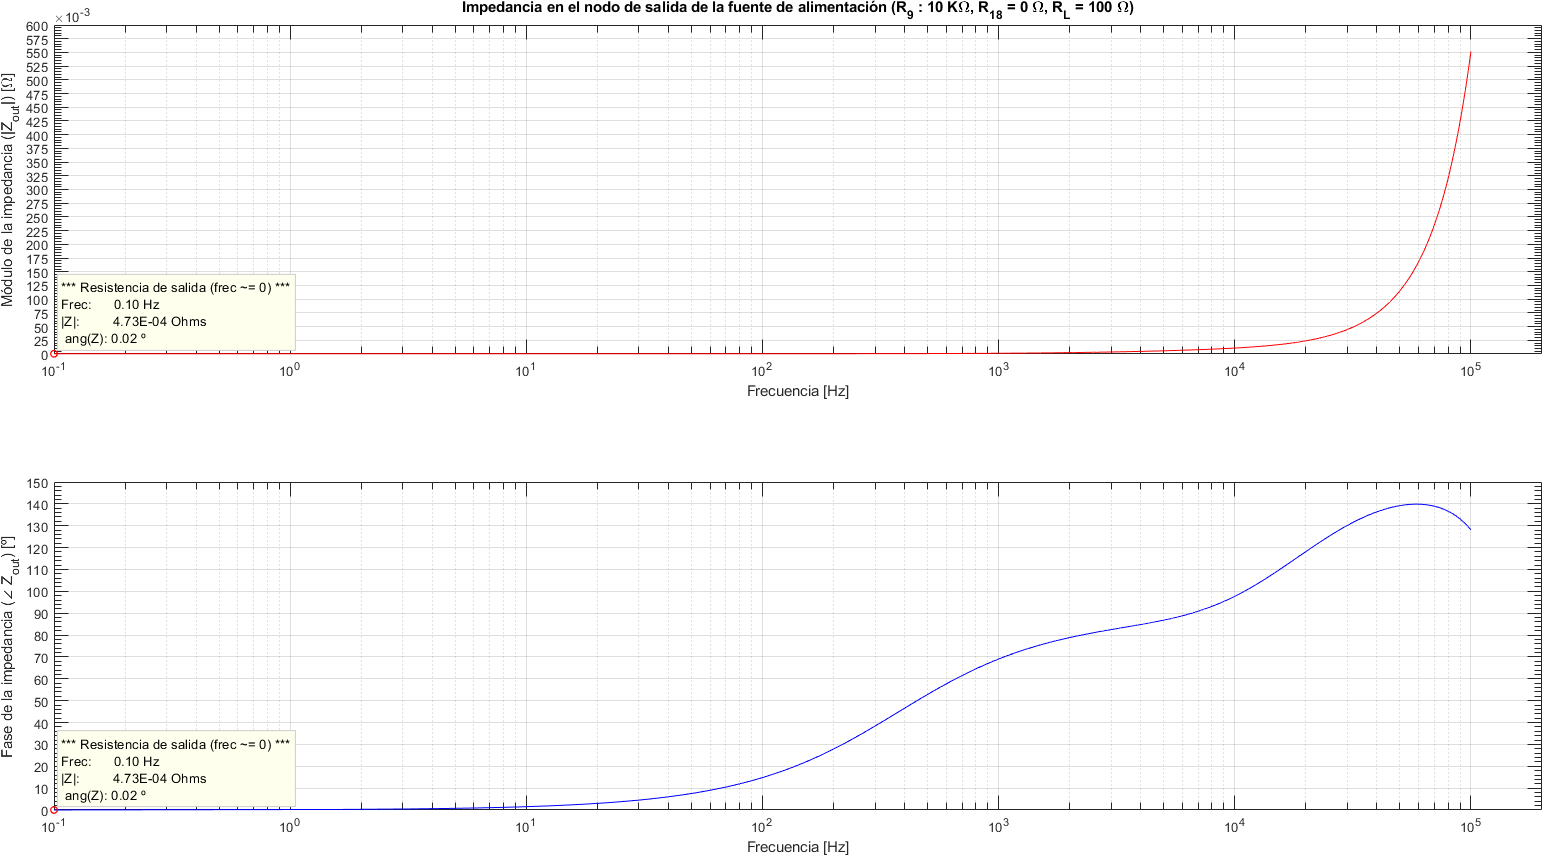
\includegraphics[width=1.2 \textwidth, angle=90]{./img/preguntas/p13.png}
\caption{\label{fig:fig_p13_output_impedance}\footnotesize{Impedancia de salida, $Z_{o}$, en función de la frecuencia, con esta variando entre $0.1 \si[per-mode=symbol]{\hertz}$ y $100 \si[per-mode=symbol]{\kilo\hertz}$.}}
\end{center}
\end{figure}



\clearpage
